\chapter{Introducción específica} % Main chapter title

\label{Chapter2}

%----------------------------------------------------------------------------------------
%	SECTION 1
%----------------------------------------------------------------------------------------
En el siguiente capitulo se realiza una introducción a las tecnológicas utilizadas en el desarrollo de este trabajo. Estas se aplican a las distintas capas del modelo de arquitectura de IoT \textit{Internet of Things}.
\section{Protocolos de comunicación}
\label{sec:ejemplo}

Los protocolos de comunicación son estándares que se utilizan para definir la manera en la que se vinculan uno o mas dispositivos. Existe un gran número de protocolos diseñados para resolver distintas problemáticas, a continuación se detallan los utilizados en el desarrollo de este trabajo.

\subsection{SPI}

EL protocolo de comunicación SPI \textit{Serial Peripherical Interface} es un protocolo de comunicación serie, sincrónico y \textit{full duplex}. Los dispositivos sincrónicos cuentan con una señala de \textit{clock} para la sincronización de los datos enviados y recibidos. A su vez, las señales MOSI \textit{Master Output Slave Input} y MISO \textit{Master Input Slave Output} permiten la transferencia simultánea de datos entre los dispositivos, esta funcionabilidad recibe el nombre de \textit{full duplex}\citep{ARTICLE3}.

En la figura \ref{fig:SPI} se observa la conexión entre dispositivos SPI.

\begin{figure}[htbp]
	\centering
	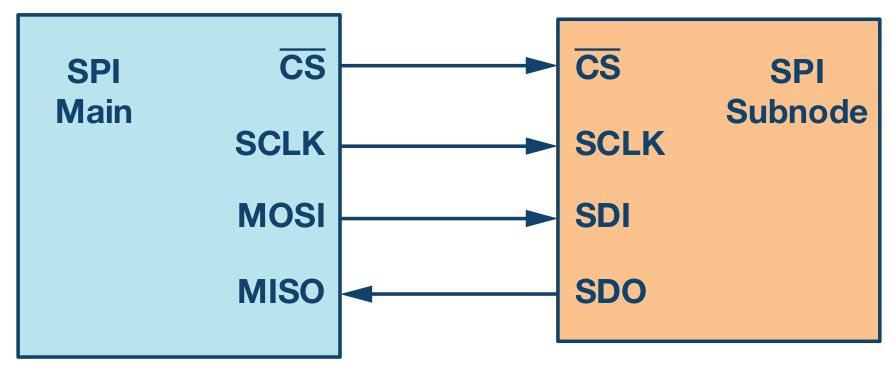
\includegraphics[width=0.6\textwidth]{./Figures/SPI.png}
	\caption{Conexión entre dispositivos SPI maestro - esclavo.}
	\label{fig:SPI}
\end{figure} 

Los dispositivos SPI pueden ser direccionables mediante las señales de CS \textit{chip select} y alcanzar velocidades de reloj de hasta 50MHz. Esto permite una gran capacidad de transferencia de datos, motivo por el cual son utilizados en dispositivos como, pantallas LCD, módulos ethernet y memorias entre otros. 


\subsection{I2C}

I2C \textit{Inter Integrated Circuit} es un protocolo de comunicación serie, sincrónico y bidireccional con un número reducido de hilos para su conexión. Se caracteriza por ser muy versátil y económico, el protocolo I2C se ha implementado en mas de 1000 circuitos integrados que han sido fabricados por mas de 50 compañías. Además, se utiliza en arquitecuras de control como SMBus   \textit{System Management Bus}, BPM    \textit{Bus Power Management Bus}, IPMI   \textit{Intelligent Platform Management Interface}, DDC   \textit{Display Data Channel} and ATCA   \textit{Advanced Telecom Computing Architecture}\citep{nxp}.

Cada dispositivo cuenta con una dirección única e inalterable para su direccionamiento. De acuerdo al tipo, pueden incorporar una o mas entradas CS \textit{chip select} para comunicarse con dispositivos idénticos sobre el mismo bus.

En la figura \ref{fig:I2C} se observa la conexión de dispositivos en un bus I2C.

\begin{figure}[htbp]
	\centering
	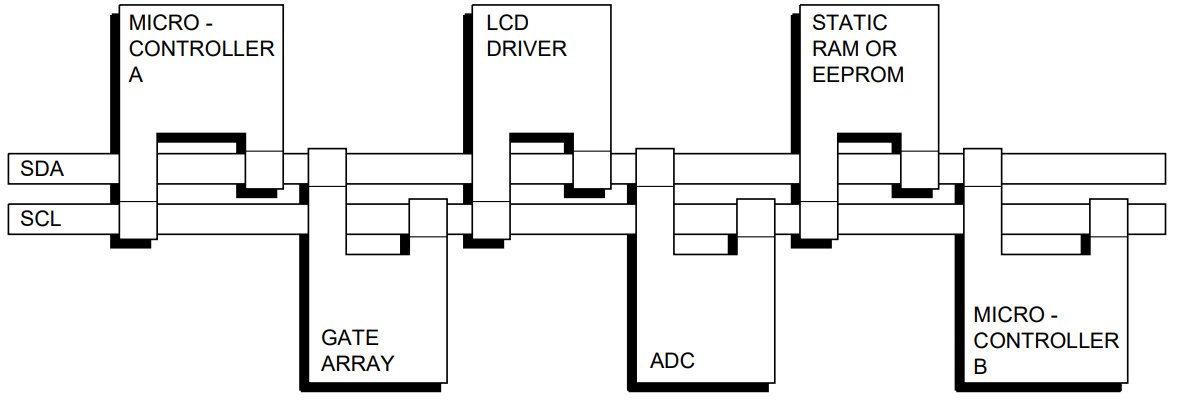
\includegraphics[width=0.8\textwidth]{./Figures/I2C.png}
	\caption{Bus de conexión de dispositivos I2C.}
	\label{fig:I2C}
\end{figure} 

Las velocidades de comunicación varían desde los 100 kHz a los 5 MHz, en la actualidad, cuentan con dispositivos para aplicaciones, militares, medicinales e industriales. Entre los más utilizados se pueden encontrar, memorias, conversores ADC, DAC, sensores de temperatura y humedad, RTC \textit{Real Time Clock}, giróscopos y otros.

\subsection{UART}

El protocolo de comunicación UART \textit{Universal Asincronous Receiver Transmitter} es uno de los más antiguos y utilizados para comunicaciones serie, este protocolo cuenta con la posibilidad de manejar 3 modos de funcionamiento:
\begin{itemize}
	\item \textit{simplex} :	El dispositivo solo envía o recibe datos.
	\item \textit{half duplex}:  El dispositivo envía y luego recibe datos.
	\item \textit{full duplex}:  El dispositivo envía y recibe datos simultáneamente.
\end{itemize}
Las conexiones entre dispositivos se realizan entre 1 transmisor y un 1 receptor, no pueden existir mas de dos dispositivos conectados, dado que no tiene capacidad de direccionamiento. En la figura \ref{fig:UART} se observa la conexión entre dispositivos USART.


\begin{figure}[htbp]
	\centering
	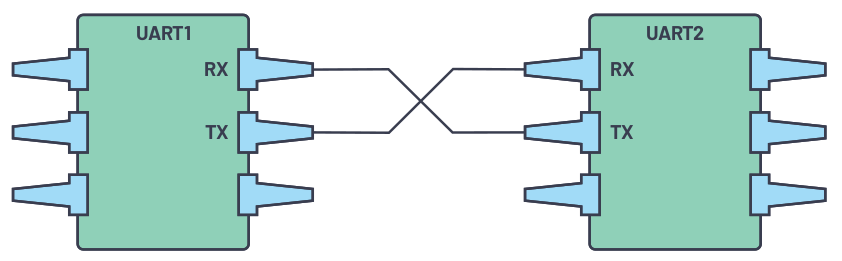
\includegraphics[width=0.4\textwidth]{./Figures/UART.png}
	\caption{Conexión entre dispositivos UART\citep{ARTICLE5}.}
	\label{fig:UART}
\end{figure} 
%https://www.analog.com/en/analog-dialogue/articles/uart-a-hardware-communication-protocol.html
%https://en.wikipedia.org/wiki/Universal_asynchronous_receiver-transmitter
El protocolo UART es utilizado en periféricos de computadora, microcontroladores, automóviles, \textit{smart cards}, SIM telefónica y otros. 
%https://en.wikipedia.org/wiki/Universal_asynchronous_receiver-transmitter


\subsection{LoRa}

LoRa \textit{Long Range} es una tecnología de comunicación inalámbrica que utiliza la modulación CSS\textit{Chip Spread Spectrum} desarrollada por la empresa Semtech. 
Este tipo de modulación posee grandes ventajas a nivel de alcance, inmunidad al ruido, seguridad y consumo de energía\citep{ARTICLE6}.

En la figura \ref{fig:LoRa} se observa la forma de onda modulada de un dispositivo LoRa. 

\begin{figure}[htbp]
	\centering
	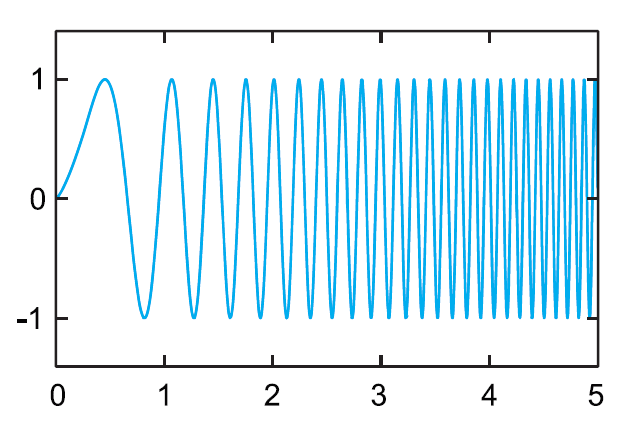
\includegraphics[width=0.3\textwidth]{./Figures/LoRa.png}
	\caption{Modulación CSS.}
	\label{fig:LoRa}
\end{figure} 

Los dispositivos LoRa utilizan el espectro de frecuencias no licenciado ISM  \textit{Industrial, Scientific and Medical} de 915 MHz en la Argentina, esto representa una ventaja frente a otras tecnologías que utilizan frecuencias licenciadas como es el caso de SigFox, NB-IoT y LTE-M.
%https://www.gotoiot.com/pages/articles/lora_intro/content.html
%https://www.semtech.com/lora/what-is-lora

%Con la incorporación del \textit{stack} LoRaWAN, la tecnología LoRa obtiene acceso a internet por medio de \textit{gateways} y un \textit{network server}, convirtiéndose en una de las mas populares del ecosistema IoT.
%
%En la figura \ref{fig:LoRaWAN} puede observarse la estructura de una red LoRaWAN.
%
%\begin{figure}[htbp]
%	\centering
%	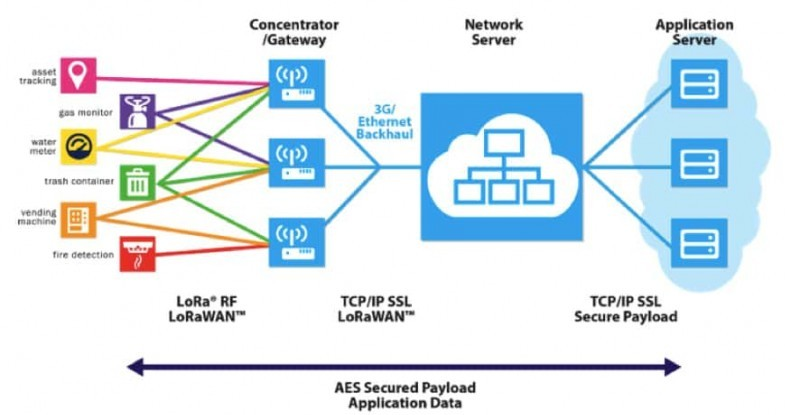
\includegraphics[width=0.8\textwidth]{./Figures/LoRaWAN.png}
%	\caption{Modulación CSS.\protect\footnotemark.}
%	\label{fig:LoRaWAN}
%\end{figure} 

En la actualidad los dispositivos LoRa sin utilizados en aplicaciones de agricultura, ciudades inteligentes, cuidado de la salud, hogar, control industrial y cadena de suministros entre otros.


\subsection{ModBUS TCP}

Modbus es un protocolo de aplicación abierto maestro-esclavo que puede ser implementado sobre distintas capas físicas.
Modbus TCP es la implementación del protocolo Modbus sobre Ethernet TCP/IP, un protocolo orientado a la conexión con el que se busca asegurar la entrega de datos. 

En la figura \ref{fig:ModBUS} puede observarse una arquitectura de comunicación ModBUS TCP en la que se combina ModBUS TCP y ModBUS Serial a través de un \textit{gateway}\citep{mbus}.

\begin{figure}[htbp]
	\centering
	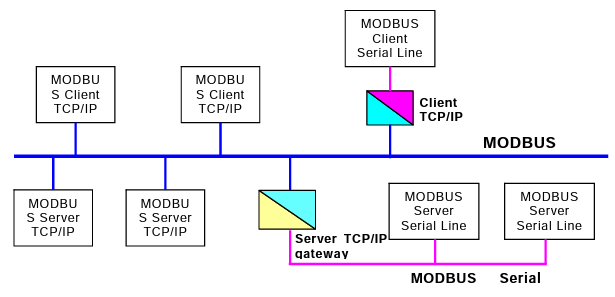
\includegraphics[width=0.7\textwidth]{./Figures/ModBUS.png}
	\caption{Arquitectura de comunicación ModBUS TCP.}
	\label{fig:ModBUS}
\end{figure} 
%MODBUS Application Protocol Specification V1.1b3
Desde su implementación, este protocolo ha sido adoptado en la industria por una gran cantidad de fabricantes. Entre los mas utilizados se pueden encontrar, controladores lógicos programables, interfases hombre máquina, sensores, actuadores, variadores de velocidad y dispositivos de campo.

ModBUS es un protocolo sencillo, económico y de rápida implementación que al día de hoy se continúa utilizando en la industria. 

\subsection{HTTP}

HTTP \textit{Hypertext Transfer Protocol} es un protocolo de la capa de aplicación utilizado para la transmisión de documentos de hipertexto como HTML \textit{HyperText Markup Language}\citep{moz1}. 

Es un protocolo del tipo cliente - servidor, en el que un cliente establece una conexión con el servidor, realiza una petición y espera la respuesta del servidor. A este mecanismo se lo denomina \textit{request/response}. 

HTTP define un conjunto de métodos de petición en el que indica la acción que se desea realizar para un recurso determinado. Entre los más utilizados se pueden encontrar, los métodos PUT, GET, POST Y DELETE\citep{moz2}. 
%https://developer.mozilla.org/es/docs/Web/HTTP/Methods

En la figura \ref{fig:HTTP} se detalle el método y la acción que se ejecuta.

\begin{figure}[htbp]
	\centering
	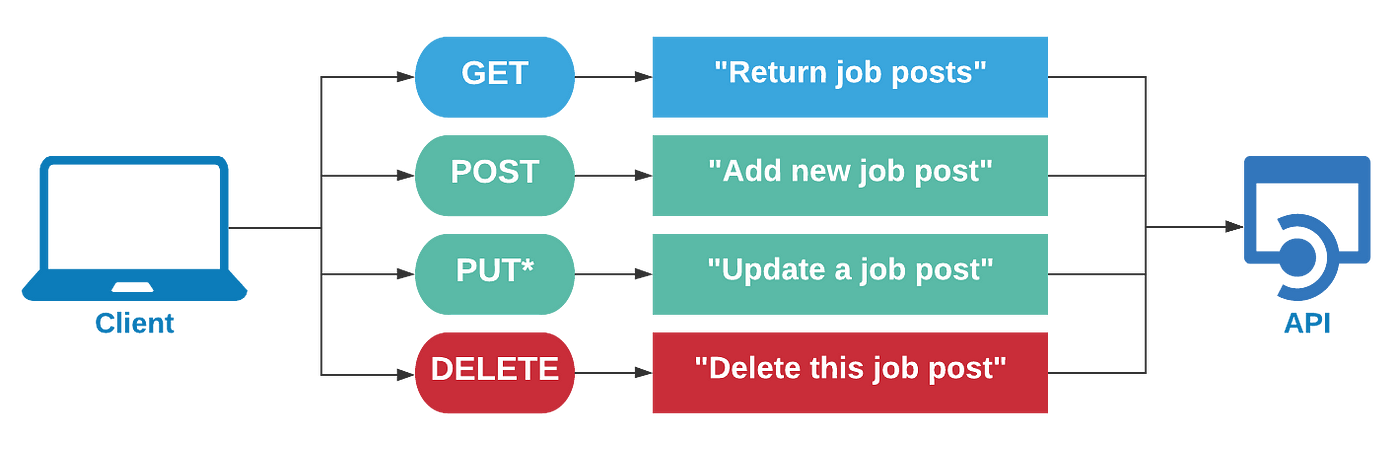
\includegraphics[width=0.6\textwidth]{./Figures/HTTP.png}
	\caption{Métodos HTTP de uso frecuente.}
	\label{fig:HTTP}
\end{figure} 

%https://miro.medium.com/v2/resize:fit:1400/1*wpbYhweLr38h8fUnuFT0Fg.png
%https://developer.mozilla.org/es/docs/Web/HTTP

En materia de seguridad, el protocolo HTTP
 puede encriptarse sobre TLS \textit{Transport Layer Security} o bien sobre SSL \textit{Secure Sockets Layer}.

\subsection{Wi-Fi}

Wi-Fi es un protocolo de red inalámbrico basado en las normas IEEE 802.11. 

Las normas IEEE 802.11 especifican los protocolos de capa física y control de acceso al medio para la implementación de una red de área local que permita la comunicación entre dispositivos. Dentro de los dispositivos que conforman una red Wi-Fi se pueden encontrar los \textit{access point} y los \textit{routers}. 

Un \textit{access point} permite que los dispositivos inalámbricos se conecten a la red inalámbrica. El \textit{access point} toma el ancho de banda proveniente de un router y lo extiende para que muchos dispositivos puedan conectarse a la red desde distancias más lejanas.

Un \textit{router} inalámbrico, también llamado router Wi-Fi, combina las funciones de red de un router y un punto de acceso inalámbrico. Un router conecta las redes locales a otras redes locales o a Internet\citep{wifii}.

El uso de los recursos de internet se encuentra en constante crecimiento, los servicios de \textit{streaming}, aplicaciones móviles y redes sociales generan mas contenidos y de mayor calidad. Estos servicios demandan un mayor ancho de banda, lo que representa un desafío para las tecnologías disponibles adaptarse a los nuevos requerimientos.

En la figura \ref{fig:WIFIEVO} se observa la evolución de la tecnología Wi-Fi.

%https://softwarelab.org/es/blog/que-es-wi-fi/
%https://en.wikipedia.org/wiki/IEEE_802.11
%https://techunwrapped.com/know-the-characteristics-and-speed-of-the-new-wifi-7-or-802-11be/
%https://www.cisco.com/c/es_mx/products/wireless/what-is-wifi.html#~preguntas-y-respuestas
%https://www.cisco.com/c/es_mx/products/wireless/wireless-router.html

\begin{figure}[htbp]
	\centering
	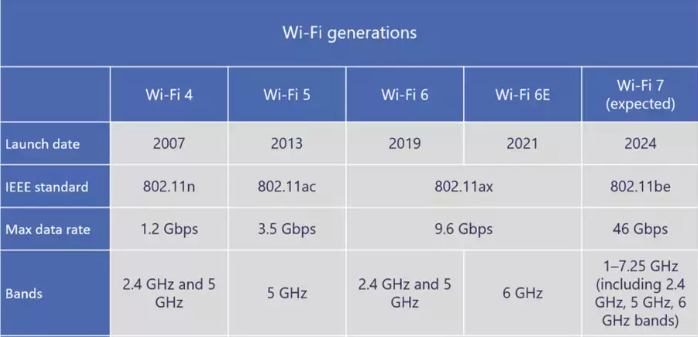
\includegraphics[width=0.7\textwidth]{./Figures/WIFIEVO.png}
	\caption{Evolución de la tecnología Wi-Fi.\protect\footnotemark.}
	\label{fig:WIFIEVO}
\end{figure} 

\footnotetext{Imagen tomada de \url{https://techunwrapped.com/know-the-characteristics-and-speed-of-the-
new-wifi-7-or-802-11be}}
%wifi_esencial
En la actualidad, la tecnología Wi-Fi se encuentra disponible en un gran número de dispositivos hogareños, industriales y \textit{weareables}. Estos dispositivos son utilizados diariamante, convirtiéndose en un recurso esencial para el desarrollo de las actividades cotidianas.

\subsection{MQTT}
%https://aws.amazon.com/es/what-is/mqtt/
El protocolo MQTT \textit{Message Queuing Telemetry Transport} tiene sus orígenes en el año 1999 en la industria del petróleo y gas. El monitoreo de los oleoductos se realizaba vía satélite, esto requería de un protocolo con ancho de banda bajo y consumo de baterías mínimo.

El protocolo MQTT se basa en los principios del modelo de publicación y subscripción. Un cliente publica datos sobre un tópico, el broker los recibe y los envía a los clientes que estén subscriptos a ese tópico. Los tópicos son la forma en que los mensajes se filtran y organizan jerárquicamente.

En la figura \ref{fig:MQTT} se detalla el modelo de publicación y subscripción.


\begin{figure}[htbp]
	\centering
	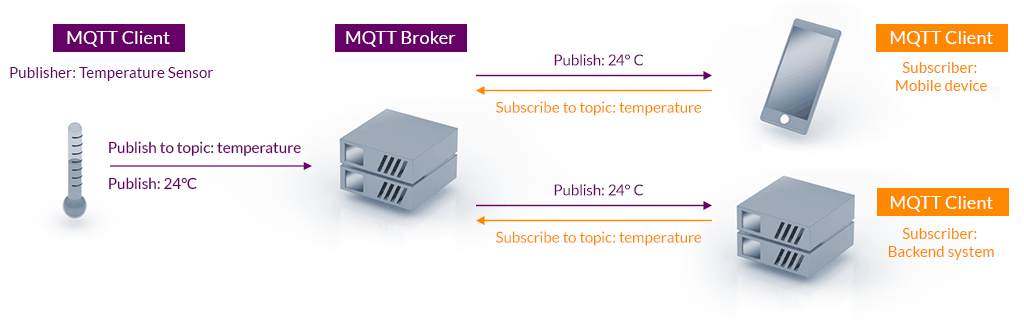
\includegraphics[width=0.8\textwidth]{./Figures/MQTT.png}
	\caption{Modelo de publicación y subscripción.\protect\footnotemark.}
	\label{fig:MQTT}
\end{figure} 
\footnotetext{Imagen tomada de \url{https://mqtt.org/assets/img/mqtt-publish-subscribe.png}}
%image https://mqtt.org/assets/img/mqtt-publish-subscribe.png

A nivel de seguridad, utiliza el protocolo SSL para proteger los datos, implementar identidad y autenticación entre clientes y brokers.


\newpage
\section{Tecnologías de backend}

El \textit{backend} es el desarrollo de la lógica y comunicación de servicios de una pagina web que permite disponer de los datos a ser visualizados por el usuario. Las instrucciones y consultas que el usuario realiza son procesadas por el \textit{backend} y luego visualizadas en el \textit{frontend}.

 
\subsection{NodeJS}
%https://nodejs.dev/en/learn/#an-example-nodejs-application
%https://cdn.buttercms.com/0Nh1yR6SSPwqnsKYSfHa
NodeJS es una plataforma de código abierto que ejecuta el motor de JavaScript V8 de Chrome. Las aplicaciones en NodeJS se ejecutan en un único proceso que corre en un solo hilo del procesador. 

Se utiliza el concepto de programación orientada a eventos para poder dar soporte a la concurrencia de tareas, el \textit{loop} principal \textit{Event Loop}  escucha los eventos y dispara una función \textit{callback} cuando uno de estos eventos es detectado\citep{node}. 

En la figura \ref{fig:MQTT} puede observarse la arquitectura de la plataforma NodeJS.

\begin{figure}[htbp]
	\centering
	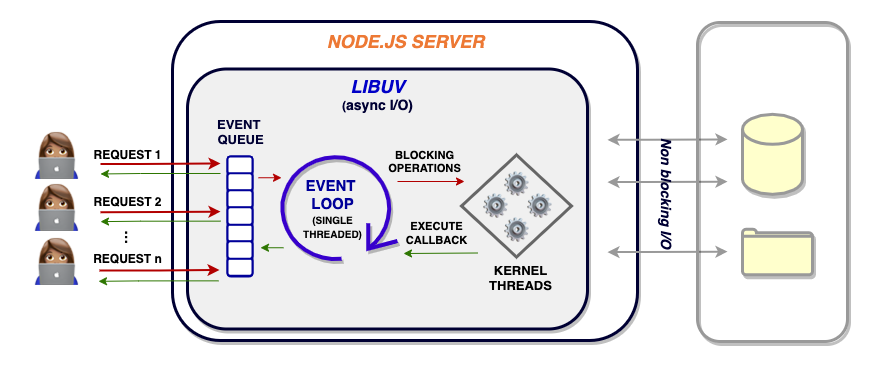
\includegraphics[width=0.8\textwidth]{./Figures/NODEJS.png}
	\caption{Arquitectura NodeJS.}
	\label{fig:NODEJS}
\end{figure}

A diferencias de otras plataformas, NodeJS consume menos recursos, todo la carga de trabajo de I/O se realiza de manera asíncrona para evitar la demora entre tareas.

\subsection{Express}
%https://www.geeksforgeeks.org/express-js/
%https://developer.mozilla.org/en-US/docs/Learn/Server-side/Express_Nodejs/Introduction
Express es un \textit{framework} que otorga funcionabilidad sobre el servidor web de NodeJS, es uno de los \textit{frameworks} más utilizados. Entre sus principales características se destacan las siguientes\citep{expr}:

\begin{itemize}
	\item Desarrollo de aplicaciones web de forma rápida y sencilla.
	\item Facilidad de configuración y uso.
	\item Definición de  rutas de aplicaciones utilizando métodos HTTP y URL.
	\item Fácil integración con motores del plantillas.
	\item Especificación de \textit{middleware} para manejo de errores.
\end{itemize}



%\subsection{JWT}
%%https://www.geeksforgeeks.org/express-js/
%%https://developer.mozilla.org/en-US/docs/Learn/Server-side/Express_Nodejs/Introduction
%Express es un \textit{framework} que otorga funcionabilidad sobre el servidor web de NodeJS, es uno de los \textit{frameworks} más utilizados. Entre sus principales caracaterísticas se pueden encontar:
%
%\begin{itemize}
%	\item Desarrollo de aplicaciones web de forma rápida y sencilla.
%	\item Facilidad de configuración y uso.
%	\item Definir rutas de aplicaciones utilizando métodos HTTP y URL.
%	\item Definir rutas de aplicaciones utilizando métodos HTTP y URL.
%	\item Fácil integración con motores del plantillas.
%	\item Especificación de \textit{middleware} para manejo de errores.
%\end{itemize}
\newpage
\section{Tecnologías de frontend} 

El \textit{frontend} es la parte del desarrollo web que se encarga de la interacción, visualización y experiencia del usuario con la aplicación web.

\subsection{Ionic}
%https://ionicframework.com/docs
\textit{Ionic Framework }es un kit de desarrollo de software \textit{frontend} de código abierto para aplicaciones híbridas basado en tecnologías web HTML, CSS y JavaScript\citep{ioni1}.
%https://ionic.io/docs/platform

Ionic permite la creación de aplicaciones para iOS, Android y la web desde un único código. Esto es posible gracias a Capacitor, un \textit{framework} para el desarrollo de aplicaciones multiplataforma que implementa las aplicaciones como una página web local.

Capacitor permite convertir cualquier proyecto web en una aplicación nativa de iOS o Android, cuenta con una librería de \textit{plugins} nativos que habilitan el acceso a distintos dispositivos y características del sistema operativo\citep{ioni2}.

En la figura \ref{fig:capacitor} se visualiza el modelo de aplicación capacitor.

\begin{figure}[htbp]
	\centering
	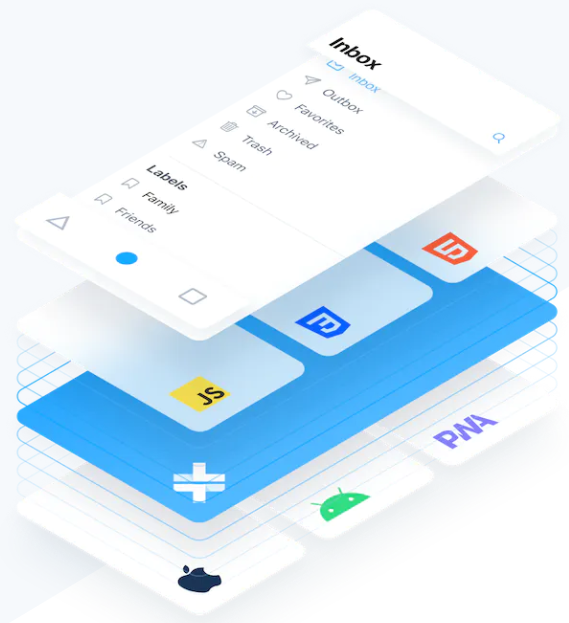
\includegraphics[width=0.4\textwidth]{./Figures/capacitor.png}
	\caption{Modelo de aplicación capacitor.}
	\label{fig:capacitor}
\end{figure}

Ionic cuenta también con una serie de herramientas para el desarrollo de la interfaz de usuario UI, entre las que se pueden encontrar, tarjetas, botones, formularios, animaciones y otros.
Estos componentes trabajan con los \textit{frameworks} React, Angular y Vue.


\subsection{Highcharts}

\textit{Highcharts} es una librería de gráficos desarrollada en JavaScript, se caracteriza por su  facilidad de integración en la página web, sus opciones de configuración y tipo de gráficos.

En la figura \ref{fig:highcharts}  puede observarse una vista reducida de los gráficos disponibles.
\newpage
\begin{figure}[htbp]
	\centering
	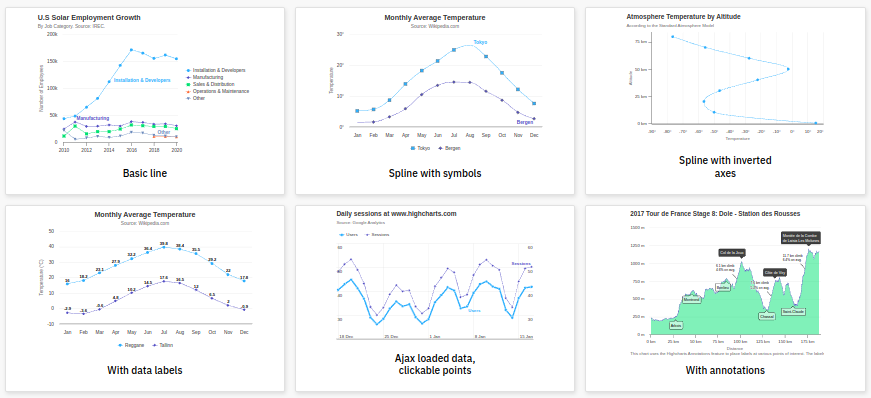
\includegraphics[width=0.9\textwidth]{./Figures/highcharts.png}
	\caption{Gráficos disponibles en librería \textit{Highcharts}.\protect\footnotemark.}
	\label{fig:highcharts}
\end{figure}

Otra herramienta muy útil para la representación de variables son los indicadores, estos son muy utilizados para la visualización de métricas en páginas relacionadas con servicios IoT.

En la figura \ref{fig:highcharts2} puede observarse una vista de los distintos tipos de indicadores.

\begin{figure}[htbp]
	\centering
	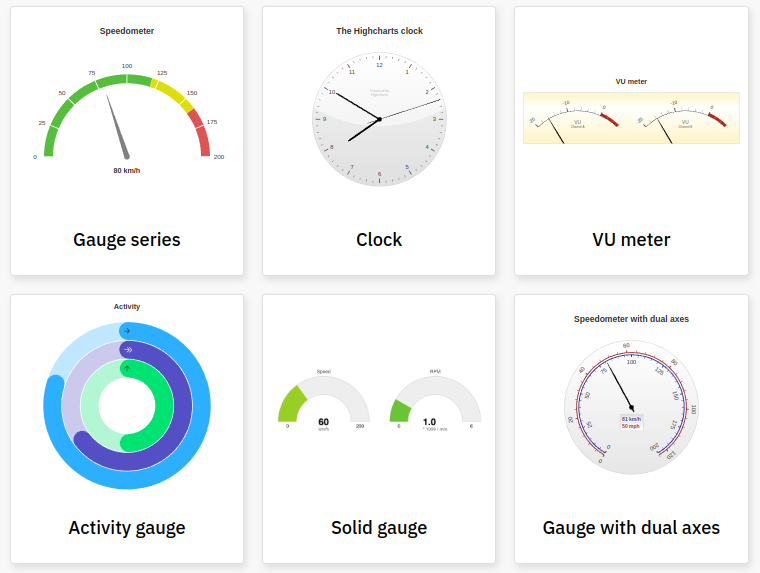
\includegraphics[width=0.8\textwidth]{./Figures/highcharts2.png}
	\caption{Indicadores disponibles en librería \textit{Highcharts}}
	\label{fig:highcharts2}
\end{figure}

\section{Dispositivos \textit{baremetal}}

Los dispositivos \textit{baremetal} son dispositivos de baja capacidad de procesamiento, son utilizados en la capa de percepción del modelo IoT para la implementación de sensores y recolección de datos.

\subsection{ESP32}
%https://www.espressif.com/en/products/socs/esp32

ESP32 es un SoC \textit{System On Chip} desarrollado por la compañía Espressif, el concepto de SoC es la integración de distintos componentes en el mismo circuito integrado, con esto se busca reducir la cantidad de componentes externos y mejorar el funcionamiento del sistema.

Los componentes que integran en SoC son los siguientes\citep{esp}:

\begin{itemize}
	\item Microprocesador doble núcleo de 32 bits.
	\item Modulo WiFi + Bluetooth de 2,4 GHz.
	\item Modulo Bluetooth LE.
	\item Selectores de antena.
	\item RF Balun.
	\item Amplificador de potencia.
	\item Amplificador de recepción de bajo ruido.
	\item Filtros.
	\item Módulos de manejo de potencia.
\end{itemize}

%El SoC es un chip que requiere de un cantidad de componentes mínimos para su funcionamiento, Espressif desarrolló los módulos ESP32 que integran en un circuito impreso los componentes necesarios para disponer de todas las prestaciones del SoC. Estos módulos cuentan con acceso a las GPIO, cristal, memoria y antena.

Espressif facilitó la implementación de sus SoCs mediante la creación de módulos, estos módulos cuentan con el SoC, la memoria de programa, los cirstales y la antena montados en un circuito impreso listo para su uso. 

En la figura \ref{fig:ESP1} puede observarse el módulo ESP-WROOM32 con el SoC y sus componentes, por otro lado en la figura \ref{fig:ESP2} se observa el módulo montado en una placa que permite el acceso a sus periféricos y cuenta con una interfaz USB-SERIE para su programación.

%\begin{figure}[htbp]
%	\centering
%	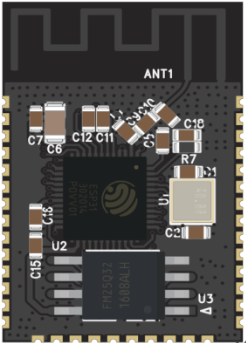
\includegraphics[width=0.3\textwidth]{./Figures/ESPMOD.png}
%	\caption{Módulo ESP-WROOM-32}
%	\label{fig:ESPMOD}
%\end{figure}
%
%\begin{figure}[htbp]
%	\centering
%	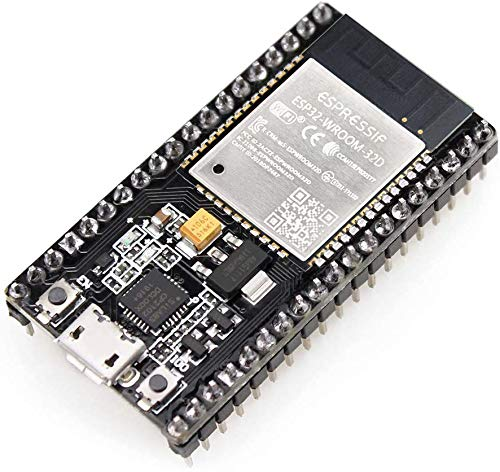
\includegraphics[width=0.3\textwidth]{./Figures/ESP322.jpg}
%	\caption{Módulo ESP-WROOM-32}
%	\label{fig:ESPMOD}
%\end{figure} 

\begin{figure}[h!]
\centering
\begin{subfigure}[b]{0.2\linewidth}
	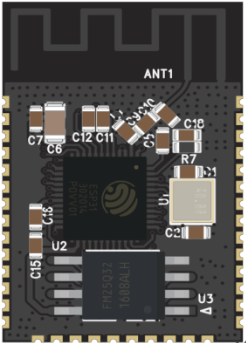
\includegraphics[width=\linewidth]{./Figures/ESPMOD.png}
	\caption{Módulo ESP-WROOM32}
	\label{fig:ESP1}
\end{subfigure}\hspace{25mm}
\begin{subfigure}[b]{0.3\linewidth}
	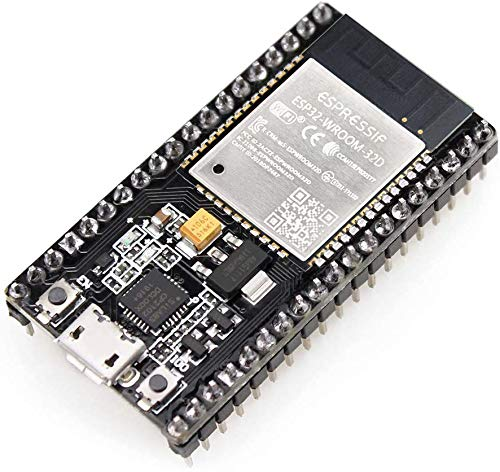
\includegraphics[width=\linewidth]{./Figures/ESP322.jpg}
	\caption{Módulo ESP-WROOM32 montado en placa desarrollo}
	\label{fig:ESP2}
\end{subfigure}
\caption{Montaje de módulo ESP32}
\label{fig:ESP32}
\end{figure}

\subsection{STM32}
%https://www.st.com/en/microcontrollers-microprocessors/stm32-32-bit-arm-cortex-mcus.html
STM32 es una familia de microcontroladores desarrolados por la compañía ST que utiliza la arquitectura ARM-Cortex. A diferencia del ESP32, este microprocesador tiene la memoria integrada en el mismo chip\citep{stm}.

Existen placas de desarrollo que cuentan con este tipo de microcontrolador, en estas se incorpora la conexión de sus entradas y salidas, fuente de alimentación, cristal de reloj, cristal de tiempo real, conector USB y pines para su programación y verificación. 

En la figura \ref{fig:bpill} se visualiza una placa de desarrollo que utiliza este microcontrolador, a esta placa se la conoce con el nombre de \textit{blackpill}.
%\newpage
\begin{figure}[htbp]
	\centering
	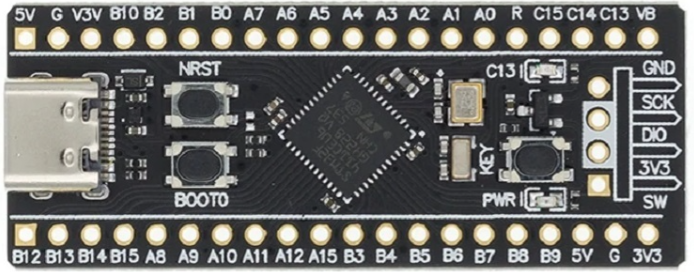
\includegraphics[width=0.5\textwidth]{./Figures/bpill.png}
	\caption{Módulo STM32}
	\label{fig:bpill}
\end{figure} 

El módulo no tiente una estructura de SoC de comunicación, por lo que estas funciones se realizan con módulos adicionales.
En la figura \ref{fig:ESP32} se observan módulos de comunicación Wi-Fi, Ethernet y LoRa.
\begin{figure}[h!]
\centering
\begin{subfigure}[b]{0.2\linewidth}
	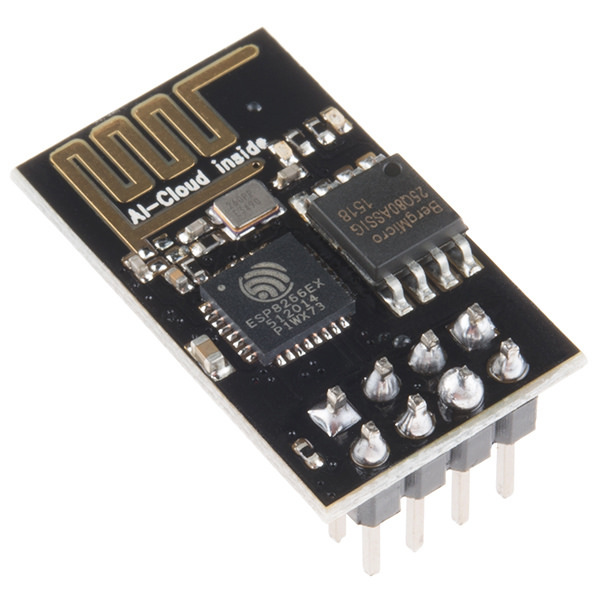
\includegraphics[width=\linewidth]{./Figures/ESP8266.jpg}
	\caption{Módulo Wi-Fi ESP8266}
	\label{fig:ESP8266}
\end{subfigure}\hspace{15mm}
\begin{subfigure}[b]{0.2\linewidth}
	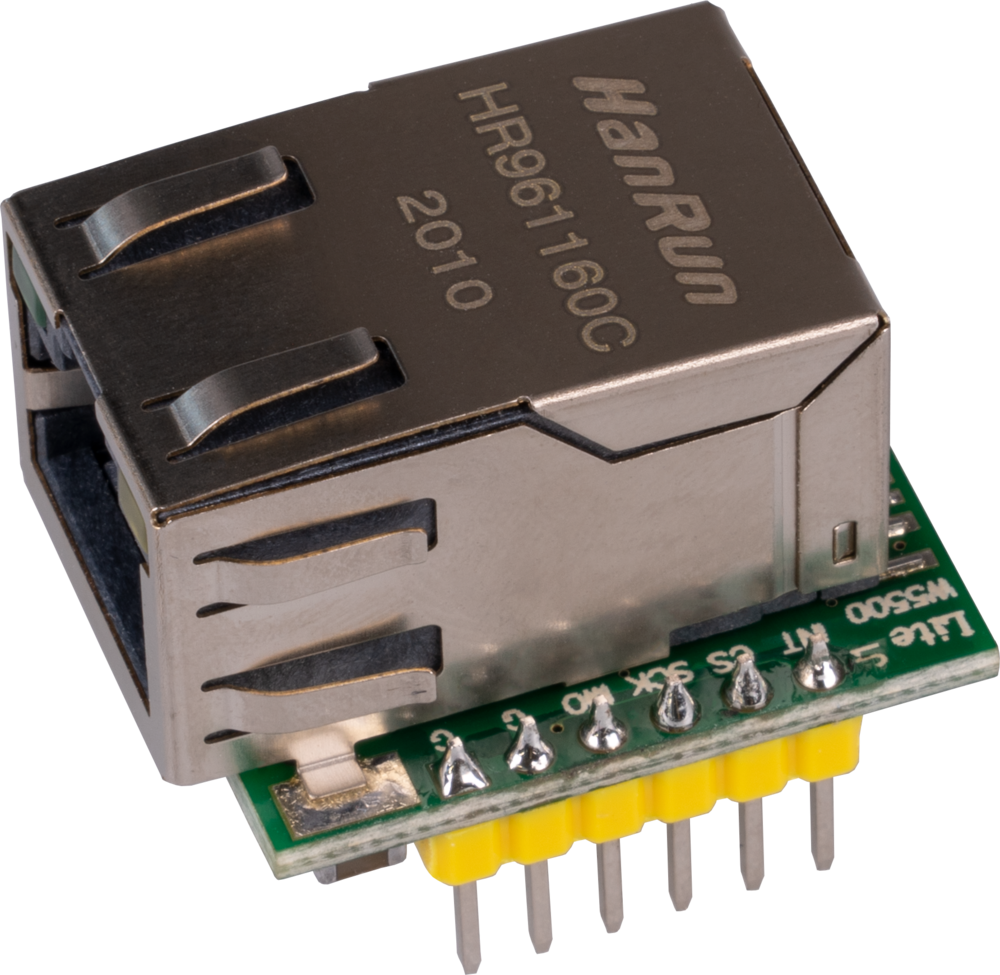
\includegraphics[width=\linewidth]{./Figures/w5500.png}
	\caption{Módulo Ethernet W5500 SPI}
	\label{fig:w5500}
\end{subfigure}\hspace{15mm}
\begin{subfigure}[b]{0.15\linewidth}
	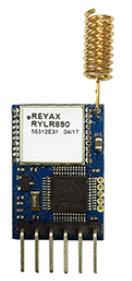
\includegraphics[width=\linewidth]{./Figures/RYLR.png}
	\caption{Módulo LoRa RYLR896}
	\label{fig:RYLR}
\end{subfigure}
\caption{Módulos de comunicación adicionales}
\label{fig:ESP32}
\end{figure}

\section{Herramientas utilizadas}

En la desarrollo de este trabajo se utilizaron herramientas de software que permitieron la programación del \textit{backend}, \textit{frontend}, base de datos y los dispositivos \textit{baremetal}. Además se utilizó software para el testeo del \textit{backend}, simulación de datos y escucha de tráfico de red para la verificación de los mensajes enviados.

\subsection{Visual Studio Code}
%https://code.visualstudio.com/docs
Visual Studio Code es un editor de código liviano compatible con Windows, iOS y Linux. Este editor tiene la posibilidad de agregar extensiones específicas para distintos lenguajes y aplicaciones\citep{vscode}.

En el desarrollo del presente trabajo se utilizan las siguientes extensiones:

\begin{itemize}
	\item C/C++ Extensions: Utilizada para la escritura de programa en lenguaje C.
	\item Espressif IDF: Herramienta para la programación de dispositivos ESP32.
	\item Docker: Herramienta para facilitar la creación y manejo de contenedores.
	\item Angular Essentials : Utilizado para la programación del frontend.
	\item Ionic:  Herramienta para el desarrollo en Ionic y Capacitor
\end{itemize}

\subsection{STM32 Cube IDE}
%https://www.st.com/en/development-tools/stm32cubeide.html
STM32 Cube IDE es un entorno de desarrollo de C/C++ basado en Eclipse®/CDT™ para la programación, configuración de periféricos, generación, compilación y depuración de código de microcontroladores STM32\citep{stcode}.

La conexión para programar y depurar el programa en el microcontrolador se realiza a través de una interfaz ST-LINKV2 USB.

En la figura \ref{fig:STLINK} se observa la interfaz de programación STLINK V2.

 \begin{figure}[htbp]
	\centering
	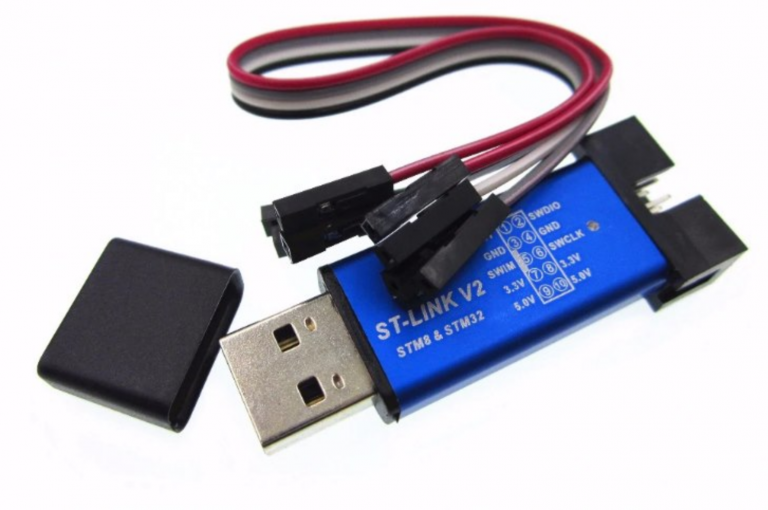
\includegraphics[width=0.5\textwidth]{./Figures/STLINK.png}
	\caption{Interfaz STLINK V2}
	\label{fig:STLINK}
\end{figure} 

\subsection{Postman}
%https://www.postman.com/
Postman es una interfaz de programación de aplicaciones que contiene herramientas para acelerar el diseño, prueba y verficación de las aplicaciones que se encuentran en desarrollo\citep{post}.

Postman se utilizó para la prueba y verificación de los \textit{endpoints} del \textit{backend}.

\subsection{phpMyAdmin}
%https://www.phpmyadmin.net/
phpMyAdmin es un software gratuito desarrollado en php que se utiliza para la administración de bases de datos MySQL y MariaDB. Soporta un amplio rango de operaciones de uso frecuente como la administración de la bases de datos, tablas, columnas, relaciones, índices, usuarios y permisos entre otros\citep{php}.

Una herramienta muy utilizada en el desarrollo de este trabajo fue la representación gráfica de las consultas SQL realizadas al \textit{backend.}

\subsection{Wireshark}
%https://www.wireshark.org/docs/wsug_html_chunked/Preface.html

Wireshark es un software de análisis de protocolos de red, soporta todo tipo de protocolos y permite la selección de las interfaces de red sobre las cuales se pretende analizar el tráfico\citep{wire}. 

Wireshark fue utilizado como herramienta de verificación para el estudio de los protocolos HTTPS y MQTTS.


